% !TEX root = ../thesis.tex

\chapter{Bezpečnostná analýza}


Pre dosiahnutie robustného riešenia sme museli zvážiť bezpečnostnú stránku programu.
Z tohto dôvodu sme vykonali bezpečnostnú analýzu.
Na vykonanie analýzy sme namodelovali diagram hrozieb pomocou nástroja Microsoft Threat Modeling Tool.
Na obrázku \ref{bez_di} je tento diagram.
Pomocou tohto programu sme veľmi rýchlo odhalili bezpečnostné hrozby, ktoré by mohli ohroziť vykonávanie nášho programu a dáta používateľa.
Ďalej v tejto kapytole popisujeme výstup našej analýzy.

\section{Zhrnutie modelu hrozby}

\begin{figure}[!t] 
	\centering 
	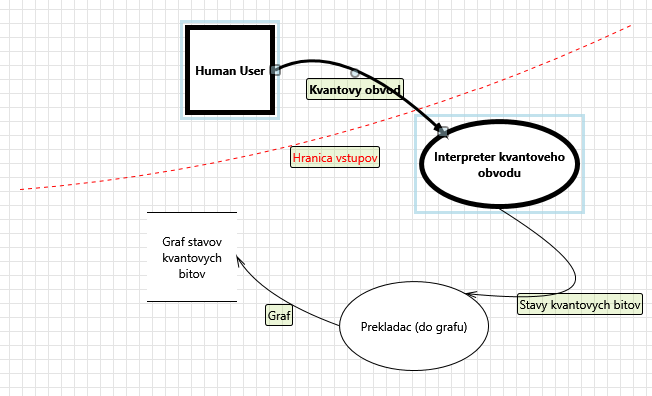
\includegraphics[width=.8\textwidth]{figures/diagram.png} 
	\caption{Diagram modelu hrozieb}
    \label{bez_di}
\end{figure}

\begin{enumerate}

\item \textbf{Spoofing cieľového dátového úložiska Graf stavov kvantovych bitov} \\ 
\textbf{Stav:} migrácia implementovaná \\
\textbf{Priorita:} vysoká
\begin{itemize}

\item[] \textbf{Kategória:} \\
Spoofing je, keď proces alebo entita je niečo iné ako jej nárokovaná identita. Medzi príklady patrí nahradenie procesu, súboru, webovej stránky alebo sieťovej adresy.
\item[] \textbf{Opis:} \\
Graf stavov kvantovych bitov môže útočník spoofovať, a to môže viesť k tomu, že údaje sa zapíšu do cieľa útočníka namiesto grafov kvantovych bitov. Zvážte použitie štandardného autentifikačného mechanizmu na identifikáciu cieľového úložiska údajov.
\item[] \textbf{Odôvodnenie:} \\
Použitie hashov na autentifikáciu.
\end{itemize}

\item \textbf{Potenciálna nadmerná spotreba zdrojov pre Prekladac (do grafu) alebo Graf stavov kvantovych bitov} \\
\textbf{Stav:} Vyžaduje sa vyšetrovanie \\
\textbf{Priorita:} vysoká 

\begin{itemize}
\item[] \textbf{Kategória:} \\
Odopretie služby nastane, keď proces alebo dátové úložisko nie je schopné obsluhovať prichádzajúce žiadosti alebo vykonávať špecifikácie.
\item[] \textbf{Opis:}  \\
Vykonáva prekladac (do grafu) alebo graf stavov kvantovych bitov výslovné kroky na kontrolu spotreby zdrojov? Útoky na spotrebu zdrojov môžu byť ťažko zvládnuteľné a niekedy je rozumné nechať OS robiť svoju prácu. Dávajte pozor, aby vaše žiadosti o zdroje neboli zablokované a aby nevypršali časové limity.
\item[] \textbf{Odôvodnenie:} \\
<neposkytuje sa migrácia>
\end{itemize}

\item \textbf{Podvádzanie externého subjektu - ľudského používateľa} \\
\textbf{Stav:} migrácia implementovaná \\
\textbf{Priorita:} vysoká 

\begin{itemize}
\item[] \textbf{Kategória:} \\
Spoofing je, keď proces alebo entita je niečo iné ako jej nárokovaná identita. Medzi príklady patrí nahradenie procesu, súboru, webovej stránky alebo sieťovej adresy.
\item[] \textbf{Opis:} \\
Ľudský užívateľ môže byť spoofovaný útočníkom a to môže viesť k neoprávnenému prístupu k interpretátoru kvantoveho obvodu. Zvážte použitie štandardného autentifikačného mechanizmu na identifikáciu externej entity.
\item[] \textbf{Odôvodnenie:} \\
Použitie autentifikácie.
\end{itemize}

\item \textbf{Nadväznosť pomocou zosobnenia} \\
\textbf{Stav:} migrácia implementovaná \\
\textbf{Priorita:} vysoká

\begin{itemize}
\item[] \textbf{Kategória:} \\
Subjekt používateľa získava zvýšenú spôsobilosť alebo privilégium využitím chyby implementácie.
\item[] \textbf{Opis:} \\
Interpreter kvantoveho  obvodu môže byť schopný zosobniť kontext ľudského používateľa, aby získal ďalšie privilégiá.
\item[] \textbf{Odôvodnenie:} \\
ACL
\end{itemize}

\item \textbf{Spoofing procesu interpretera kvantoveho obvodu} \\
\textbf{Stav:} migrácia implementovaná \\
\textbf{Priorita:} vysoká

\begin{itemize}
\item[] \textbf{Kategória:} \\
Spoofing je, keď proces alebo entita je niečo iné ako jej nárokovaná identita. Medzi príklady patrí nahradenie procesu, súboru, webovej stránky alebo sieťovej adresy.
\item[] \textbf{Opis:} \\
Interpreter kvantoveho obvodu môže útočník spoofovať, čo môže viesť k poskytovaniu informácií ľudským používateľom. Zvážte použitie štandardného autentifikačného mechanizmu na identifikáciu cieľového procesu.
\item[] \textbf{Odôvodnenie:} \\
Použitie autentifikácie
\end{itemize}

\item \textbf{Potenciálne nedostatočné overenie vstupu pre Interpreter kvantoveho obvodu} \\
\textbf{Stav:} migrácia implementovaná \\
\textbf{Priorita:} vysoká

\begin{itemize}
\item[] \textbf{Kategória:} \\
Manipulácia je akt zmeny bitov. Manipulácia s procesom zahŕňa zmenu bitov v bežiacom procese. Podobne manipulácia s dátovým tokom zahŕňa zmenu bitov na drôte alebo medzi dvoma bežiacimi procesmi.
\item[] \textbf{Opis:} \\
Údajom, ktorý tečie cez Kvantovy obvod, môže útočník zmanipulovať. Môže to viesť k odmietnutiu služobného útoku na tlmočníka kvantového rozsahu alebo k zvýšeniu výsadného privilégia proti tlmočníkovi kvantového množstva alebo k sprístupneniu informácií interpretom kvantového množstva. Opomenutie overiť, či je vstup očakávaný, je hlavnou príčinou veľmi veľkého množstva problémov, ktoré možno zneužiť. Zvážte všetky cesty a spôsob spracovania údajov. Overte správnosť všetkých vstupov pomocou schváleného prístupu na overenie vstupu do zoznamu.
\item[] \textbf{Odôvodnenie:} \\
Validácia vstupu.
\end{itemize}

\item \textbf{Potenciálne odmietnutie údajov Interpretera kvantového obvodu} \\
\textbf{Stav:} migrácia implementovaná \\
\textbf{Priorita:} vysoká

\begin{itemize}
\item[] \textbf{Kategória:} \\
Hrozby odmietnutia zahŕňajú protivníka, ktorý popiera, že sa niečo stalo.
\item[] \textbf{Opis:} \\
Interpreter kvantoveho obvodu tvrdí, že nedostal údaje zo zdroja mimo hranice dôveryhodnosti. Zvážte použitie protokolovania alebo auditu na zaznamenanie zdroja, času a súhrnu prijatých údajov.
\item[] \textbf{Odôvodnenie:} \\
Audit vstupov.
\end{itemize}

\item \textbf{Sniffing toku údajov} \\
\textbf{Stav:} migrácia implementovaná \\
\textbf{Priorita:} vysoká

\begin{itemize}
\item[] \textbf{Kategória:} \\ 
Zverejňovanie informácií nastane, keď ich môže prečítať neoprávnená strana.
\item[] \textbf{Opis:} \\
Údaj, ktorý tečie cez Kvantovy obvod, môže útočník vyvolať. V závislosti od toho, aký typ údajov môže útočník prečítať, možno ho použiť na útok na iné časti systému alebo jednoducho na odhalenie informácií vedúcich k porušeniu súladu. Zvážte šifrovanie toku údajov.
\item[] \textbf{Odôvodnenie:} \\ 
Ručné zadávanie.
\end{itemize}

\item \textbf{Potenciálne zlyhanie procesu alebo zastavenie Interpretera kvantoveho obvodu} \\ 
\textbf{Stav:} migrácia implementovaná \\
\textbf{Priorita:} vysoká

\begin{itemize}
\item[] \textbf{Kategória:} \\
Odopretie služby nastane, keď proces alebo dátové úložisko nie je schopné obsluhovať prichádzajúce žiadosti alebo vykonávať špecifikácie.
\item[] \textbf{Opis:} \\ 
Tlmočník kvantoveho signálu havaruje, zastavuje, ukončuje alebo beží pomaly; vo všetkých prípadoch porušujúcich metriku dostupnosti.
\item[] \textbf{Odôvodnenie:} \\
Využívanie kvót na predchádzanie veľkým vstupom.
\end{itemize}

\item \textbf{Tok údajov Kvantový obvod je potenciálne prerušený} \\
\textbf{Stav:} migrácia implementovaná \\
\textbf{Priorita:} vysoká

\begin{itemize}
\item[] \textbf{Kategória:} \\
Odopretie služby nastane, keď proces alebo dátové úložisko nie je schopné obsluhovať prichádzajúce žiadosti alebo vykonávať špecifikácie.
\item[] \textbf{Opis:} \\
Externý agent preruší údaje tečúce cez hranice dôveryhodnosti v oboch smeroch.
\item[] \textbf{Odôvodnenie:} \\
Validácia používateľa
\end{itemize}

\item \textbf{Interpreter kvantoveho obvodu môže byť predmetom zvýšenia oprávnenia pomocou vzdialeného vykonávania kódu} \\
\textbf{Stav:} migrácia implementovaná \\
\textbf{Priorita:} vysoká

\begin{itemize}
\item[] \textbf{Kategória:} \\
Subjekt používateľa získava zvýšenú spôsobilosť alebo privilégium využitím chyby implementácie.
\item[] \textbf{Opis:} \\ 
Ľudský užívateľ môže byť schopný diaľkovo vykonať kód pre tlmočníka kvantoveho kontroly.
\item[] \textbf{Odôvodnenie:} \\ 
Validácia vstupu.
\end{itemize}

\item \textbf{Vyzdvihnutie zmenou realizačného toku v Interpretore kvantoveho obvodu}  \\
\textbf{Stav:} migrácia implementovaná \\
\textbf{Priorita:} vysoká

\begin{itemize}
\item[] \textbf{Kategória:}  \\
Subjekt používateľa získava zvýšenú spôsobilosť alebo privilégium využitím chyby implementácie.
\item[] \textbf{Opis:} \\ 
Útočník môže preniesť údaje do kvantového interpreta Interpreter, aby zmenil tok vykonávania programu v Interpretore kvantového obvodu podľa výberu útočníka.
\item[] \textbf{Odôvodnenie:} \\ 
Overenie vstupných údajov.
\end{itemize}

\item \textbf{Vyzdvihnutie pomocou zosobnenia} \\ 
\textbf{Stav:} migrácia implementovaná \\
\textbf{Priorita:} vysoká

\begin{itemize}
\item[] \textbf{Kategória:} \\
Subjekt používateľa získava zvýšenú spôsobilosť alebo privilégium využitím chyby implementácie.
\item[] \textbf{Opis:} \\
Prekladač (do grafu) môže byť schopný zosobniť kontext interpretátora kvantovehobvodu, aby získal ďalšie privilégium.
\item[] \textbf{Odôvodnenie:} \\
Nastavenie povolení pre Prekladač (do grafu).
\end{itemize}

\end{enumerate}

\section{Zhrnutie}

Pri analýze sme odhalili 13 hrozieb.
Z hoto sa nám úspešne podarilo vyriešiť 12.
Pomocou tejto metódy sa nám veľmi rýchlo podarilo nájsť a eliminovať bezpečnostné nedostatky nášho programu.
